\documentclass[10pt]{article}

\usepackage{polski}
\usepackage[utf8]{inputenc}
\usepackage{graphicx}
\usepackage{amsmath}
\usepackage{amssymb}
\DeclareMathVersion{varbold}
\author{Przemysław Sankowski}
\date{19.01.2018}
\title{Badanie przebiegu zmienności funkcji}


\begin{document}
\maketitle
\noindent
\tableofcontents
\newpage


\section{Wprowadzenie}
Żeby uzyskać przebieg zmienności funkcji należy wyznaczyc: \\ \\
1. Dziedzinę. \\
2. Miejsca zerowe. \\
3. Punkt przecięcia z osią Oy. \\
4. Granice na krańcach dziedziny. \\
5.Asymptoty. \\
6.Przedziały monotoniczności. \\
7.Ekstrema. \\
8.Przedziały wklęsłości i wypukłości. \\
9.Punkty przegięcia. \\ \\ \\
Do badania powyższych własności używamy drugiej pochodnej funkcji.
Na końcu rysujemy wykres funkcji i odczytujemy z niego zbiór wartości funkcji. \\ \\
Na przykład rozwiązania weźmy funkcję: 
{\large \begin{equation*}
f(x)=\frac{1}{x^{2}-2} + 1
\end{equation*}}
\newpage


\section{Wyznaczenie dziedziny funkcji}
{\large \begin{eqnarray}
x^2 - 2 = 0 \\
x^2 = 2 \\
\label{dziedzina} x = - \sqrt{2} \hspace{0.5cm} \vee \hspace{0.5cm} x = \sqrt{2}
\end{eqnarray}} \\
A zatem dziedzina funkji to:
{\large \begin{equation*}
\mathbb{R}\backslash\{-\sqrt{2},\sqrt{2}\}
\end{equation*}}


\section{Wyznaczenie miejsc zerowych funkcji}
{\large \begin{eqnarray}
\frac{1}{x^2 - 2} + 1 = 0 \\
\frac{1}{x^2 -2} = 1 \\
1 = -(x^2 -2) \\
x^2 = 1 \\
x = 1 \hspace{0.5cm} \vee \hspace{0.5cm} x = -1
\end{eqnarray}}


\section{Wyznaczenie punktu przecięcia z osią Oy}
{\large \begin{equation}
f(0) = \frac{1}{0^2 -2} + 1 = \frac{1}{-2} + 1 = -\frac{1}{2} + 1 = \frac{1}{2} 
\end{equation}}
\\ 
Zatem punkt przecięcia z osią Oy to:
{\large \begin{equation*}
\left( 0,\frac{1}{2} \right)
\end{equation*}}

\newpage

\section{Wyznaczenie granic dziedziny}
Należy wyznaczyć granice funkcji w $+\infty$ \ i $-\infty$ oraz dla x'ów przerywających ciągłość funkcji, czyli dla krawędzi tej części funkcji, która znajduje się poza dziedziną. W naszym przypadku to $x=\sqrt{2}$ i $x=- \sqrt{2}$ (\ref{dziedzina}). \\
Zacznijmy od granic w nieskończonościach:

{\large \begin{equation} \label{aspoz1}
\lim_{n \to +\infty}f(x) = \lim_{n \to +\infty} \left( \frac{1}{x^2 - 2} +1 \right) = \left[ \frac{1}{+\infty} + 1 \right] = [ 0 + 1 ] = 1
\end{equation}
\begin{equation} \label{aspoz2}
\lim_{n \to -\infty}f(x) = \lim_{n \to -\infty} \left( \frac{1}{x^2 - 2} +1 \right) = \left[ \frac{1}{-\infty} + 1 \right] = [ 0 + 1 ] = 1
\end{equation}} \\

\noindent Otrzymujemy w ten sposób asymptotę poziomą wyrażoną wzorem $y=1$. Teraz obliczamy granicę w punktach nieciągłości. Zacznijmy od granicy lewostronnej z $\sqrt{2}$:

{\large \begin{eqnarray}
\lim_{x\to\sqrt{2}^-}f(x) = \lim_{x\to\sqrt{2}^-} \left( \frac{1}{x^2 - 2} +1 \right) = \left[ \frac{1}{\sqrt{2}^- -2} + 1 \right] = \left[ \frac{1}{0^-} + 1 \right] = \\ = [-\infty +1] = -\infty \phantom{\hspace{6.6cm}} \nonumber
\end{eqnarray}} \\

\noindent Następnie granicę prawostronną z $\sqrt{2}$:

{\large \begin{eqnarray}
\lim_{x\to\sqrt{2}^+}f(x) = \lim_{x\to\sqrt{2}^+} \left( \frac{1}{x^2 - 2} +1 \right) = \left[ \frac{1}{\sqrt{2}^+ -2} + 1 \right] = \left[ \frac{1}{0^+} + 1 \right] = \\ = [+\infty +1] = +\infty \phantom{\hspace{6.6cm}} \nonumber
\end{eqnarray}} \\

\noindent Ze względu na to, że granice wyliczone w powyższych równaniach są różne, granica dla $x = \sqrt{2}$ nie istnieje. \\
Następnie należy wyliczyć granicę dla $x=-\sqrt{2}$:

{\large \begin{eqnarray}
\lim_{x\to -\sqrt{2}^-}f(x) = \lim_{x\to -\sqrt{2}^-} \left( \frac{1}{x^2 - 2} +1 \right) = \left[ \frac{1}{ -\sqrt{2}^+ -2} + 1 \right] = \left[ \frac{1}{ 2^+ -2} + 1 \right] =  \\ = \left[ \frac{1}{0^+} + 1 \right] = [+\infty +1] = +\infty \phantom{\hspace{5.75cm}}
\end{eqnarray}} \\

{\large \begin{eqnarray}
\lim_{x\to -\sqrt{2}^+}f(x) = \lim_{x\to -\sqrt{2}^+} \left( \frac{1}{x^2 - 2} +1 \right) = \left[ \frac{1}{ -\sqrt{2}^+ -2} + 1 \right] = \left[ \frac{1}{0^-} + 1 \right] = \\ = [-\infty +1] = -\infty \phantom{\hspace{7.2cm}} \nonumber
\end{eqnarray}} \\

\noindent Granica dla $x = - \sqrt{2}$ również nie istnieje.

\section{Wyznaczenie asymptot}

{\bf Asymptoty pionowe} to proste pionowe przechodzące przez punkty nieciągłości funkcji, czyli znajdujące się w $x=-\sqrt{2}$ i $x=\sqrt{2}$ (\ref{dziedzina})

\noindent {\bf Asypmtoty poziome} istnieją, jeżeli granice w $+\infty$ i $-\infty$ istnieją i nie są nieskończone. Z równań (\ref{aspoz1}) i (\ref{aspoz2}) wynika, że asymptota pionowa istnieje, a jej wartość to $y=1$.

\noindent W tym przykładzie {\bf asymptoty ukośne} nie istnieją, ale normalnie wyznaczamy je wzorami: 
{\large \begin{eqnarray*}
\lim_{x\to +\infty}\frac{f(x)}{x} = a \\
\lim_{x\to +\infty}(f(x)-ax) = b \\
\end{eqnarray*}} \\

\noindent Jeśli obie te granice są skończone, to {\bf asymptota ukośna prawostronna} opisana jest równaniem:
{\large \begin{equation*}
y = ax + b
\end{equation*}

Tak samo obliczamy {\bf asymptotę ukośną lewostronną}, tylko że liczymy granice w $-\infty$. \newpage


\section{Wyznaczenie przedziałów monotoniczności}
Aby wyznaczyć przedziały monotoniczności (oraz ekstrema) musimy obliczyć pochodną funkcji.
{\large \begin{equation} \label{pochodna}
f'(x) = \left(\frac{1}{x^2 - 2} + 1\right)' = \frac{-2x}{(x^2-2)^2}
\end{equation}

\noindent Aby policzyć pochodną skorzystaliśmy ze wzorów z \cite{wzorki} 
Funkcja f(x) jest {\bf rosnąca} jeśli $f'(x) > 0$, {\bf malejąca} natomiast kiedy $f'(x) < 0$, należy więc rozwiązać obie te nierówności. 

{\large \begin{eqnarray}
f'(x) > 0 \rightarrow \frac{-2x}{(x^2 - 2)}^2 > 0 \rightarrow -2x > 0 \rightarrow x < 0 \\
f'(x) < 0 \rightarrow \frac{-2x}{(x^2 - 2)}^2 < 0 \rightarrow -2x < 0 \rightarrow x > 0
\end{eqnarray}}

\noindent Z powyższych równań wynika, że funkcja jest rosnąca dla \\ $x \in (-\infty; 0)$, a malejąca dla $x \in (0;+\infty)$
\section{Wyznaczenie ekstremów}
\noindent Do obliczenia ekstremów potrzebujemy pochodnej, którą wyliczyliśmy już w równaniu \ref{pochodna}. Funkcja może mieć ekstremum tylko w tych miejscach gdzie jej pochodna się zeruje. Dodatkowo aby ekstremum istniało, to funkcja musi w danym punkcie zmienić monotoniczność. Mogą być dwie sytuacje: \\ \\
$\circ$ Jeśli funkcja była rosnąca i w pewnym momencie zaczyna maleć, to mamy ekstremum maksimum (wykres lokalnie przypomina górkę) \\
$\circ$ Jeśli funkcja była malejąca i w pewnym momencie zaczyna rosnąć, to mamy ekstremum minimum (wykres lokalnie przypomina dolinę) \\
Zaczynamy od znalezienia x'ów dla których $f'(x) = 0$, liczymy więc.
{\large \begin{equation}
f'(x) = 0 \rightarrow \frac{-2x}{(x^2 - 2)}^2 = 0 \rightarrow -2x = 0 \rightarrow x = 0
\end{equation}}
Następnie należy sprawdzić, czy funkcja w punkcie $x=0$ zmienia monotoniczność. \\
Ustaliliśmy już, że dla $x \in (-\infty; 0)$ funkcja f(x) jest rosnąca, a dla $x \in (0;+\infty)$ - malejąca, zatem jest to ekstremum minimum, którego wartość należy wyliczyć z równania f(0):
{\large \begin{equation}
f'(0) = \frac{1}{0^2 -2}+1 = -\frac{1}{2} +1 = \frac{1}{2}
\end{equation}}
\section{Wyznaczenie przedziałów wklęsłości i wypukłości}
Aby wyznaczyć przedziały wklęsłości i wypukłości (oraz punkty przegięcia), to musimy obliczyć drugą pochodną funkcji. Zatem liczymy:
{\large \begin{equation}
f''(x) = \left(\frac{-2x}{(x^2-2)^2}\right)' = \dots = \frac{6x^4 - 8x^2 -8}{(x^2 -2)^4}
\end{equation}}
Ponownie skorzystaliśmy z wzorów z \cite{wzorki} \\
Funkcja f(x) jest {\bf wypukła} kiedy $f''(x) > 0$, a {\bf wklęsła} kiedy $f''(x) < 0$. \\
Na początku wyznaczymy przedziały w których funkcja jest wypukła, czyli rozwiążemy nierówność:
{\large \begin{eqnarray}
f''(x) > 0 \rightarrow \frac{6x^4 - 8x^2 -8}{(x^2 -2)^4} > 0 \rightarrow 6x^4 - 8x^2 -8 > 0 \rightarrow \\ \rightarrow 6x^4 - 8x^2 -8 = 0 \rightarrow t=x^2 [t>0] \rightarrow 6t^2 - 8t - 8 = 0 \nonumber \\
\triangle = 64 - 4 * 6 * (-8) = 256 \nonumber \\
\sqrt{\triangle} = 16 \nonumber \\
t_1 = -\frac{8}{12} < 0 \nonumber \\
t_2 = 2 < 0 \nonumber \\
x^2 = 2 \rightarrow x = \sqrt{2} \cup x = -\sqrt{2} \nonumber 
\end{eqnarray}
Zatem miejsca zerowe funkcji $y = 6x^4 - 8x^2 - 8$ to $-\sqrt{2}$ i $\sqrt{2}$
Następnie musimy naszkicować wykres tej funkcji (Rysunek \ref{fig:Wykres}). \\
\begin{figure} \begin{center}
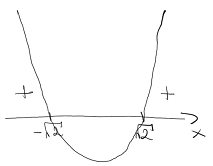
\includegraphics[width=6cm]{przyklad1a}
\caption{Piękny wykresik}
\label{fig:Wykres}
\end{center}
\end{figure} $$ $$
\noindent Z wykresu możemy odczytać gdzie funkcja jest większa od 0, z czego otrzymujemy: \\
$6x^4 - 8x^2 - 8 > 0$ dla $ x \in (-\infty; -\sqrt{2})\cup(\sqrt{2}; +\infty)$ \\
To znaczy, że funkcja jest wypukła dla $ x \in (-\infty; -\sqrt{2})\cup(\sqrt{2}; +\infty)$. Również z wykresu możemy wywnioskować, że funkcja jest wklęsła dla $ x \in (-\sqrt{2}; \sqrt{2})$
\section{Wyznaczenie punktów przegięcia}
Punkty przegięcia występują w tych miejscach, w których funkcja zmienia wypukłość. Żeby je znaleźć, to należy rozwiązać równanie:
{\large \begin{equation}
f''(x) = 0
\end{equation}}
Z równania (23) wynika, że $x = -\sqrt{2} \cup x=\sqrt{2}$. \\
Oznacza to, że w tych punktach funkcjaa zmienia wypukłość, czyli teoretycznie są to punkty przegięcia, ale... Niestety nie należą one do dziedziny - na początku wyliczyliśmy, że dziedzina to: $\mathbb{R}\backslash\{-\sqrt{2},\sqrt{2}\}$. Z czego płynie wniosek, że nasza funkcja f(x) nie ma punktów przegięcia. \\ \\
Na koniec rysujemy jeszcze wykres funkcji i odczytujemy z niego zbiór wartości. \\
\begin{figure} \begin{center}
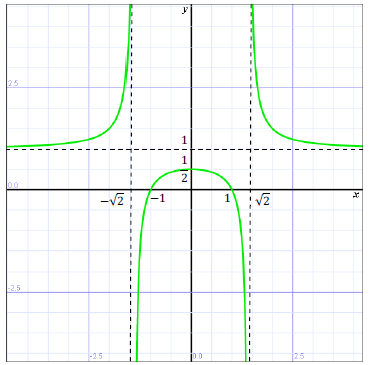
\includegraphics[width=9cm]{przyklad1b}
\caption{Wykres całej funkcji}
\label{fig:Funkcja}
\end{center}
\end{figure}
Zgodnie z (Rysunek \ref{fig:Funkcja} - następna strona) zbiór wartości funkcji to:
{\large \begin{equation}
\left(-\infty; \frac{1}{2}\right)\cup(1;+\infty)
\end{equation}}

Artykuł napisany na podstawie \cite{matematyka}

\bibliography{bibliografia}
\bibliographystyle{plain}
\end{document}
